

In this section we study another fairness notion, {\equitability} (formally defined below), which requires the ex-ante utilities of the agents to be equalized by a mechanism that is BIC, IIR, ex ante WBB. We show that even with zero-value seller, the seller ex-ante utility in an {\equitable} mechanism (that is BIC, IIR, ex ante WBB) might be arbitrary lower than the maximum ex ante utility of the seller (which is at most the maximum utility of the buyer). Additionally, for every $\eps > 0$, the GFT of an {\equitable} mechanism might be only an $\eps$ fraction of the {\SecondBest} $\OPTSB$.

\defequitability*

\begin{figure}
    \centering
    \subfloat[]{
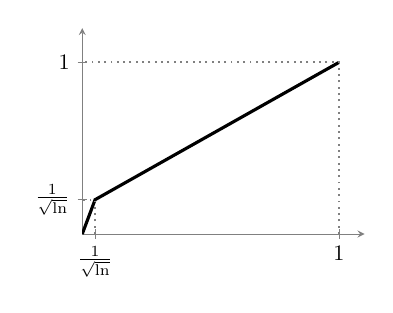
\begin{tikzpicture}[scale=0.8, transform shape]
\begin{axis}[
axis line style=gray,
axis lines=middle,
xlabel = $\quant$,
ylabel = $\revcurve$,
xtick={0, 0.05, 1},
ytick={0, 0.2, 1},
xticklabels={0, $\frac{1}{\constantH\sqrt{\ln\constantH}}$, 1},
yticklabels={0, $\frac{1}{\sqrt{\ln\constantH}}$, 1},
xmin=0,xmax=1.1,ymin=-0.0,ymax=1.2,
width=0.5\textwidth,
height=0.4\textwidth,
samples=1000]


\addplot[black!100!white, line width=0.5mm] (0, 0) -- (0.05, 0.2) -- (1, 1);


\addplot[dotted, gray, line width=0.3mm] (1, 0) -- (1, 1) -- (0, 1);
\addplot[dotted, gray, line width=0.3mm] (0.05, 0) -- (0.05,0.2) -- (0, 0.2);



\end{axis}

\end{tikzpicture}
\label{fig:equitable:revenue curve}
}~~~~
    \subfloat[]{
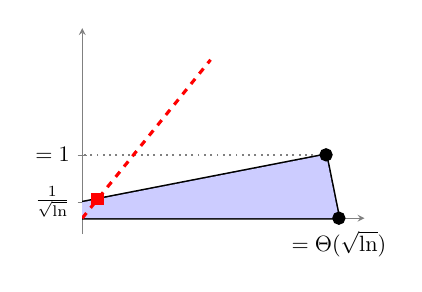
\begin{tikzpicture}[scale=0.8, transform shape]
\begin{axis}[
axis line style=gray,
axis lines=middle,
xlabel = $\buyerexanteutil$,
ylabel = $\sellerexanteutil$,
xtick={0, 1},
ytick={0, 0.1, 0.4},
xticklabels={0, $\buyerbenchmark=\Theta(\sqrt{\ln\constantH})$},
yticklabels={0, $\frac{1}{\sqrt{\ln\constantH}}$, $\sellerbenchmark = 1$},
xmin=0,xmax=1.1,ymin=-0.1,ymax=1.2,
width=0.5\textwidth,
height=0.4\textwidth,
samples=1000]


\addplot[black!100!white, line width=0.5mm] (0, 0) -- (0, 0.1) -- (0.95, 0.4) -- (1, 0) -- (0, 0);

\fill[blue!20] (0, 0) -- (0, 0.1) -- (0.95, 0.4) -- (1, 0) -- (0, 0);



\addplot[dotted, gray, line width=0.3mm] (0.9, 0.4) -- (0, 0.4);

\addplot[dashed, red, line width = 0.5mm] (0, 0) -- (0.5, 1);

\draw[black, fill=black, line width=0.5mm] (axis cs:1, 0) circle[radius=0.08cm];
\draw[black, fill=black, line width=0.5mm] (axis cs:0.95, 0.4) circle[radius=0.08cm];

% \draw[red, fill=red, line width=0.5mm] (axis cs:0.06, 0.12) circle[radius=0.08cm];

\draw[red, fill=red, line width=0.5mm] (0.04, 0.09) rectangle (0.08, 0.15);

\end{axis}

\end{tikzpicture}
\label{fig:equitable:ex ante utility pair}
}
\caption{Graphical illustration of \Cref{example:equitable}. In \Cref{fig:equitable:revenue curve}, the black curve is the revenue curve of the buyer. In \Cref{fig:equitable:ex ante utility pair}, the shaded region corresponds to the pair of buyer and seller's ex ante utilities $(\buyerexanteutil,\sellerexanteutil)$ that is achievable from some BIC, IIR, ex ante WBB mechanism. The two black points represent the traders' ex ante utility pair induced by the {\BuyerOffer} and {\SellerOffer}, respectively. The red dashed line represents equitable utility pairs (i.e., ones with $\buyerexanteutil = \sellerexanteutil$). The red square corresponds to the GFT-optimal {\equitable} mechanism, whose GFT and two traders' ex ante utilities are significantly worse than the {\SecondBest} $\OPTSB$ and two traders' own benchmarks $\buyerbenchmark,\sellerbenchmark$.}
    \label{fig:equitable}
\end{figure}


We consider the following instance where the seller has a deterministic value of zero, and the buyer has a regular valuation distribution.
\begin{example}
    \label{example:equitable}
    Fix any $\constantH \geq e$. The buyer has a regular valuation distribution $\buyerdist$, which has support $[1, \constantH]$ and cumulative density function $\buyercdf(\val) = \frac{(\constantH\sqrt{\ln\constantH} - 1)(\val - 1)}{(\constantH\sqrt{\ln\constantH} - 1)(\val - 1) + \constantH - 1}$ for $\val \in[1,\constantH]$
    and $\buyercdf(\val) = 1$ for $\val \in(\constantH, \infty)$.
    (Namely, there is an atom at $\constantH$ with probability mass of $\frac{1}{\constantH\sqrt{\ln\constantH}}$.)
    The seller has a deterministic value of 0.
    See \Cref{fig:equitable} for an illustration of the revenue
curve and the bargaining set of $\buyerdist$.
\end{example}

\begin{lemma}
    \label{lem:equitable GFT UB}
    Fix any $\eps > 0$. In \Cref{example:equitable} with sufficiently large $\constantH$ (as a function of $\eps$),
    every BIC, IIR, ex ante WBB, and {\equitable} $\mech$ obtains at most $\eps^2$ fraction of the {\SecondBest} $\OPTSB$, i.e., $\GFT{\mech} \leq \eps^2 \cdot \OPTSB$. Moreover, the seller and buyer's ex ante utilities is at most $\eps$ and $\eps^2$ fraction of their benchmarks, i.e., $\sellerexanteutil(\mech) \leq \eps \cdot \sellerbenchmark$ and $\buyerexanteutil(\mech) \leq \eps^2 \cdot \buyerbenchmark$.
\end{lemma}
Recall that the (unbiased) {\RandomOffer} ({\RO}) ensures that each trader receives at least $\frac{1}{2}$ fraction of her own benchmark, i.e., $\sellerexanteutil(\RO) \geq \frac{1}{2}\cdot \sellerbenchmark$ and $\buyerexanteutil(\RO)\geq \frac{1}{2}\cdot \buyerbenchmark$. In contrast, \Cref{lem:equitable GFT UB} indicates that by imposing the {\equitability}, it may not only limit the GFT but also significantly reduce \emph{both} traders' ex ante utilities (compared with their benchmarks). In this sense, the {\equitability} is not be an appropriate fairness definition, since it may be disliked by both traders (due to low ex ante utilities) and the social planner (due to low GFT).

\begin{proof}[Proof of \Cref{lem:equitable GFT UB}]
    Let $\constantH = \max\{e^{4/\eps^2},e^{49}\}$. In \Cref{example:equitable}, the {\SecondBest} $\OPTSB$ can be computed as 
    \begin{align*}
        \OPTSB = \expect[\val]{\val} = 
        \displaystyle\int_1^{\constantH}\val\cdot \d \buyercdf(\val) + \constantH\cdot (1 - \buyercdf(\constantH)) \geq  
        \sqrt{\ln\constantH}
        =
        \frac{2}{\eps}
    \end{align*}
    Meanwhile, two traders' benchmarks are $\sellerbenchmark = 1$ and $\buyerbenchmark = \expect[\val]{\val} \geq \frac{2}{\eps}$. 
    
    Fix any BIC, IIR, ex ante WBB, and {\equitable} mechanism $\mech = (\alloc, \price, \sellerprice)$. We consider two cases depending on expected payment $\expect[\val]{\price(\val)}$ of the buyer.

    \xhdr{Case (a) $\expect[\val]{\price(\val)} \leq 2 \sqrt{1 / \ln\constantH}$:} In this case, since mechanism $\mech$ is ex ante WBB, the seller's ex ante utility can be upper bounded as 
    \begin{align*}
        \sellerexanteutil(\mech) = \sellerprice(0) \leq \expect[\val]{\price(\val)} \leq 2 \sqrt{1 / \ln\constantH} = \eps
    \end{align*}
    Moreover, since mechanism is {\equitable}, the buyer's ex ante utility can also be upper bounded as 
    \begin{align*}
        \buyerexanteutil(\mech) = \sellerexanteutil(\mech) \leq 2 \sqrt{1 / \ln\constantH} = \eps
    \end{align*}
    Putting all the pieces together, we show all three inequalities in the lemma statement, i.e.,
    \begin{align*}
        \GFT{\mech} = \expect[\val]{\price(\val)} + \buyerexanteutil(\mech)
        \leq 2\eps \leq \eps^2 \cdot \OPTSB~,
        \\
        \sellerexanteutil(\mech) \leq \eps \leq \eps\cdot \sellerbenchmark
        \;\;\mbox{and}\;\;
        \buyerexanteutil(\mech) \leq \eps \leq \eps^2\cdot \buyerbenchmark
    \end{align*}
    We finish the analysis of case~(a).
    
    \xhdr{Case (b) $\expect[\val]{\price(\val)} \geq 2\sqrt{1/\ln\constantH}$:} In this case, we argue that mechanism $\mech$ violates the {\equitability}. (In other words, this case never happens.) Invoking \Cref{prop:revenue equivalence}, we obtain
    \begin{align*}
        \expect[\val]{\price(\val)} = \expect[\val]{\virtualval(\val)\cdot \alloc(\val)} = \virtualval(\constantH)\cdot (1 - \buyercdf(\constantH))\cdot \alloc(\constantH) 
        +
        \displaystyle\int_{1}^\constantH \virtualval(\val)\cdot \alloc(\val)\cdot\d \buyercdf(\val)
    \end{align*}
    Combining with the facts that $\virtualval(\constantH)\cdot (1 - \buyercdf(\constantH))\cdot \alloc(\constantH)  \leq \sqrt{1/\ln\constantH}$ and $\expect[\val]{\price} \geq 2\sqrt{1/\ln\constantH}$, we obtain
    \begin{align*}
        \displaystyle\int_{1}^\constantH \virtualval(\val)\cdot \alloc(\val)\cdot\d \buyercdf(\val)
        \geq \frac{1}{2}\cdot \expect[\val]{\price(\val)}
    \end{align*}
    Next, we upper bound the ex ante utility of the buyer as follows
    \begin{align*}
        \buyerexanteutil(\mech) &{} = \expect[\val]{\val\cdot \alloc(\val) - \price(\val)}
        \geq 
        \int_1^\constantH \val\cdot \alloc(\val)\cdot \d\buyercdf(\val) - 
        \expect[\val]{\price(\val)}
        \\
        &{}\overset{(a)}{\geq}
        \frac{1}{2}\left(1 - \sqrt{\frac{1}{\ln\constantH}}\right)\cdot \expect[\val]{\price(\val)}\cdot \sqrt{\ln\constantH} - \expect[\val]{\price(\val)} \overset{(b)}{\geq} 2 \cdot \expect[\val]{\price(\val)}
    \end{align*}
    where inequality~(a) holds since $\int_1^\constantH\virtualval(\val)\alloc(\val)\cdot\d\buyercdf(\val) \geq \expect[\val]{\price(\val)}/2$ argued above and the buyer's interim allocation $\alloc(\val)$ is weakly increasing in $\val$ (due to BIC), and inequality~(b) holds since $\constantH\geq e^{49}$. Meanwhile, since mechanism $\mech$ is ex ante WBB, the seller's ex ante utility is at most 
    \begin{align*}
        \sellerexanteutil(\mech) = \sellerprice(0) \leq \expect[\val]{\price(\val)} \leq \frac{1}{2}\cdot \buyerexanteutil(\mech) < \buyerexanteutil(\mech)
    \end{align*}
    which implies mechanism $\mech$ violates the {\equitability}. This is a contradiction. Therefore, we finish the analysis of case (b) and the proof of \Cref{lem:equitable GFT UB}.
\end{proof}
